\documentclass{amsart}
\usepackage{amsfonts} % For math fonts
\usepackage{amsmath, amssymb, amsthm}
\usepackage{float}
\usepackage{enumitem}
\usepackage{graphicx}
\usepackage{listings} % For custom coding font
\usepackage{xcolor}

\lstset{
    language=Python,
    backgroundcolor=\color{gray}, % Light gray background
    basicstyle=\ttfamily\small\color{white}, % Code style
    keywordstyle=\color{cyan}\bfseries, % Keywords style
    stringstyle=\color{yellow}, % Strings style
    commentstyle=\color{black}, % Comments style
    frame=single, % Box around code
    rulecolor=\color{white}, % Frame color
    numbers=left, % Line numbers
    numberstyle=\tiny\color{white}, % Line number style
    breaklines=true, % Automatic line breaking
    showstringspaces=false
}

\setlist[enumerate,1]{label=\arabic*.}
\setlist[enumerate,2]{label=\alph*.,itemindent=2em}
\setlist{topsep=0pt, leftmargin=*, labelsep=1em}

\title{HW5 CS 180}
\author{Asher Christian 006-150-286}
\date{ 24.02.25}

\begin{document}
\maketitle

\section{Exercise 1}
\emph{
    Given an unsorted integer array, find all pair with given difference k in it without using any
    extra space.
    arr = [1,5,2,2,2,5,5,4] k =3
    Output: (2,5) and (1,4)
}\\
I propose the following algorithm that I will later justify
{\small
    \begin{itemize}
        \item \texttt{set k to be abs(k)}
        \item \texttt{use heap sort to sort the array in place in ascending order}
        \item \texttt{initialize two pointers the first pointing at the first element and the second at the second one named first and one named second}
        \item \texttt{while the pointers are not pointing to the last element}
            \begin{itemize}
                \item \texttt{compute the difference between the elements pointed at by the pointer}
                \item \texttt{if the difference is equal to k output the values pointed at by both pointers in a pair and advance the second pointer and first pointer until they are both
                    pointing at new elements}
                \item \texttt{If the difference is greater than k advance the first pointer until it is pointing at a new element}
                \item \texttt{If the difference is less than k advance the second pointer until it is pointing at a new element}
                \item \texttt{if it any point the second pointer must advance but is incapable by the size of n, end the algorithm}
                \item \texttt{advance the second pointer if at any time it is pointing to the same element as the first pointer so they are never pointing at the same element}
            \end{itemize}
    \end{itemize}
}
I will now prove the correctness of this algorithm assuming the correctness of the heap sort which I will later analyze.
Given the sorted array first note that if $k < 0$ then any pair with difference $k$ is also a pair with difference $-k$ in the other order
so it suffices to check those pairs with $k \ge 0$. Then since $k \ge 0$ all pairs in this sorted array will have the smaller element before the larger element.
Every pair outputed by my algorithm is valid as is verified by the difference calculation. Assume for contradiction
that there is a pair $(a,b)$ in the array such that $b-a = abs(k)$ and  it is not outputted by the algorithm. Consider the first time that
the first pointer points at a, there are three cases in which this could happen. First a is the initial element in which case the second pointer is also pointing to a.
the second case is if the algorithm previously found a pair with difference k and advanced both the first and second pointers to new elements. In this case let  $(c,d)$ be the
previous pair then $c < a < d < b$ by the ordering and so the element pointed to by the second pointer is no greater than b. In the third case the difference was too large with some $c < a$ and so
the pointer was advanced to $a$. In this case the second pointer is also pointing to a value less than or equal to b for if it were not then it was pointing to an element larger than b and when it was pointing to b the difference between b and c
was too small and so the algorithm would have advanced the first pointer and kept the second poitner at b. Thus there is always a state in which a is pointed to by the first pointer
and the second pointer is pointing to a value less than or equal to $b$. If it is pointing to b it outputs (a,b) and we are done.
If it points to an element less than $b$, then the difference is less than k and so the second pointer advances. This happens repeatedly until
after a finite amount of steps the second pointer points to $b$ in which case the pair is outputted and we are done. Thus (a,b) is outputted and we are done. Note that
a must be visited by the first pointer since the first pointer visits every element such that $a-f \le k$ where f is the largest element. Note that the case where the algorithm terminates before examining every element, every
pair with largest element being the largest element of the array has been checked and so no more pairs exist.\\

Heapsort is as follows using array indexing in place of actual node storage of the heap.
{\small
    \begin{itemize}
        \item \texttt{Convert the array into a max heap}
            \begin{itemize}
                \item \texttt{For each item in the array}
                    \begin{itemize}
                        \item \texttt{while the item's parent node is smaller than it}
                            \begin{itemize}
                                \item \texttt{swap node with parent node}
                            \end{itemize}
                    \end{itemize}
            \end{itemize}
        \item \texttt{Pop off the maximum element and switch it for the last heap element to place it in final list}
            \begin{itemize}
                \item \texttt{Swap the first element of array with last element in heap}
                \item \texttt{While swapped element is not larger than both children}
                    \begin{itemize}
                        \item \texttt{swap with larger child}
                    \end{itemize}
            \end{itemize}
    \end{itemize}
}
We have covererd heaps in class so it is known that heapify works. In particular each time we add an element we add it to the bottom of the heap and then
heapify up to place it in a valid position. When the sorting stage happens we guarantee that at each step the largest element in the array not yet placed
is put at the end thus justifying a valid ordering. This algorithm takes $O(n\log n)$ time since each insertion or deletion takes $O(\log n)$ and $O(n)$ such
actions are performed.
The total running time of the algorithm is then $O(n \log n)$ dominated by the sorting. After sorting we do a linear time run through of the list as
each pointer visits every index $O(1)$ times for a total of $O(n)$ operations since the indices only increase and at least one will increase at each comparison.

additionally the space complexity is $O(1)$ since heapsort is done in place, and every comparison and swap can be one with $O(1)$ extra variables
no data structure is introduced and no recursion creates memory usage.


\section{Exercise 3 P 314}
For part (a)
consider the graph with the nodes
$v_1,v_2,v_3,v_4,v_5$
with the edges
\[
    (v_1,v_2), (v_1,v_3), (v_2,v_5), (v_3,v_4), (v_4,v_5)
.\] 
\begin{figure}[H]
    \centering
    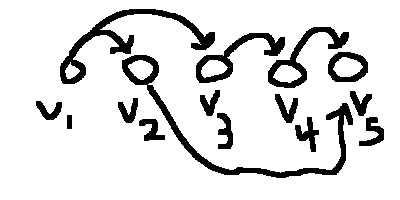
\includegraphics[width=0.8\textwidth]{example_graph.png}
\end{figure}
This algorithm would find the shortest path to be of length 2 since it greedily picks the node
with the least index. It would thus first pick the edge leading to vertex 2 and then from there the only edge possible is vertex 5.
If instead the edges $(v_1,v_3),(v_3,v_4),(v_4,v_5)$ were picked, the length would be 3.
\\
For part (b):\\
Let opt(i) be the length of the longest path to vertex $i$. For each vertex, if there are no incoming
edges then opt(i) = -inf, if there are incoming edges $opt(i) = 1 + \max_{k}\{opt(k)\}$ where $k \in \{\text{vertices with edges ending in vertex $i$}\}$. and
we set explicitely opt(0) = 0. If we compute opt(i) for each i, then opt(n) is the longest path to vertex n.
I prove the validity of this algorithm inductively.
Clearly for $v_1$ the longest path from $v_1$ to $v_1$ is zero since no edges can end on $v_1$ by the rule that every edge starts at 
a lower index than it ends at and no index is less than 1.
Inductively assume that we find the shortest path to all vertices up to $i-1$ then for vertex $i$, the longest path to vertex $i$ must pass
through an edge that goes into vertex $i$, all of those edges are ones that have been already discovered and found their longest paths by the inductive hypothesis
and thus the longest path to vertex $i$ is the longest path to a vertex that has an edge leading to vertex  $i$ plus one, which is exactly what $opt(i)$ computes. Thus $opt(i)$ is
the longest path to every vertex.
\\
The algorithm is as follows assuming for each vertex we can read off incoming edges in $O(1)$ time.
{\small
    \begin{itemize}
        \item \texttt{Initialize array of length n called opt initializing every value to -inf and the first element to 0}
        \item \texttt{For i in \{2,...,n\}}
            \begin{itemize}
                \item \texttt{Compute opt(i) = $1 + \max_k\{opt(k)\}$ where k indexes across each incoming edge incident to $v_i$}
            \end{itemize}
        \item \texttt{return opt(n)}
    \end{itemize}
}
this algorithm runs in $O(n+m)$ time, this is because it first does an $O(n)$ initialization, then for each $n$ nodes it does $O(n_v)$ work
examining $opt(k)$ for each $k$  incident edge where $n_v$ is the number of incoming edges for that node. In total it does $O(m)$ such operations on edges for a total of $O(n+m)$


\section{Exercise 5 P 316}
Let opt(i) be the largest sum attainable given the first i characters.
Consider opt(i), the ith character must be in some word, there are i possible words it can be in corresponding to all
pairs (j,i) with $1 \le j \le i$ (i,i) meaning just i indicating the start and end indices of the word. 
Let quality([j,i]) denote the quality of the string including  $x_jx_{j+1}...x_i$. Then opt(i) is 
 \[
     \max_{0 \le j \le i-1}\{opt(j)+\text{quality}([j+1,i])
.\] 
with $opt(0) = 0$.
This is true as shown by induction on the number of characters  $n$. If $n=1$ then the expression only has one term $opt(0) + \text{quality}([1,1])$ 
which is the only possible value. Inductively assume that for the first $i-1$ letters the algorithm finds the optimal sum. Then for $i$ letters,
the  ith letter must be in some word starting at index $j$ and $opt(i) = \text{quality}([j,i]) + opt(j-1)$ by inductive hypothesis since  $[j,i]$ is the optimal word
and $opt(j-1)$ is optimal by induction hypothesis. In fact our algorithm will examine every such word and settle only on the one that produces the highest sum so this ordering will be seen
and thus the algorithm will correctly identify $opt(i)$. If in addition to opt(i) we store word(i) corresponding to the $j$ value that opt(i) picks we can retain what words
are chosen optimally.

the algorithm is as follows
{\small
    \begin{itemize}
        \item \texttt{Intialize an array of length n called opt and another of length n called word and set opt(0) = 0}
        \item \texttt{For i in $\{1,2,...,n\}$}
             \begin{itemize}
                 \item \texttt{set opt(i) = $\max_{0 \le j \le i-1}\{opt(j) + \text{quality}([j+1,i])\}$ and record the j satisfying maximality}
                 \item \texttt{set word(i) = j}
            \end{itemize}
        \item \texttt{opt(n) is the maximum score}
        \item \texttt{starting at word(n) return [word(n),n] and [word(word(n)-1), word(n)-1] ... to retrieve the segments}
    \end{itemize}
} 
this algorithm operates in $O(n^2)$
time. First it creates an array in $O(n)$ time, then for each $i$ it does $O(i)$ operations for a total of $O(n^2)$ in the 
main loop. lastly recursively finding the partitions takes $O(n)$ time in worst case having to follow the word array $n$ times.

\section{Exercise 4 P 321}
For part (a) the algorithm given does not work for consider the two strings\\
A = 10, 0; B = 0, 100
This algorithm would greedily pick $a_0$ thus locking in $a_0,a_1$ which sums to 10 when the true optimal solution is $b_0,b_1$ for a total of 100.
\\
We compute the optimal solution that ends in either set A or set B at time step i, when we transition from A to B for example, the time step in which we do no work
we say we end in set B. Thus we compute
opt[i][A] and opt[i][B] for the optimal number of computations completed ending on A or B at that time step. Set opt[1][A] = $a_1$ and opt[1][B] = $b_1$.
Then for any $i$, opt[i][A] is one of the following:\\
In the optimal solution the last turn ended in A or B. If it ended in A then opt[i][A] = opt[i-1][A] + $a_i$, if it ended in B then opt[i][A] = opt[i-1][B]
similarly for opt[i][B]
opti[i][B] = max(opt[i-1][B] +  $b_i$, opt[i-1][A])
.\\
optimality of this method is proven inductively, clearly the optimal solution ending at timestep 1 is accurate since there is only one choice per set.
Assuming it holds for i-1, at time step i there are only two possiblities per set of how the optimal solution ends in the set either it completes a transition or it stays the same
both of the resulting weights are computed and the maximal one is chosen. Thus at each step optimality is preserved.

Implementing the algorithm is as follows:
{\small
    \begin{itemize}
        \item \texttt{initialize opt[A] and opt[B] n dimensional arrays with opt[A][1] = $a_1$ and opt[B][1] = $b_1$}
        \item \texttt{for i in \{2,...,n\}}
            \begin{itemize}
                \item \texttt{opt[A][i] = max\{opt[A][i-1] + $a_i$, opt[B][i-1]\}}
                \item \texttt{opt[B][i] = max\{opt[B][i-1] + $b_i$, opt[A][i-1]\}}
            \end{itemize}
        \item \texttt{return max(opt[A][n] , opt[B][n])}
    \end{itemize}
}
this algorithm runs in $O(n)$ time by doing a constant (4 comparisons and some algebra) calculations per iteration on $O(n)$ elements.

\section{Exercise 5}
\emph{Given a rod of length n inches and an array of prices that contains prices of all pieces of size smaller than n. Determine the maximum value
obtainable by cutting up the rod and selling the pieces. For example, if length of the rod is 8 and the values of different pieces are given as following, 
then the maximum obtainable value is 22 (by cutting in two pieces of lengths 2 and 6)}

if the length of the rod is 1 then there is only one value it can have namely val(1).
Assume we know the most efficient way each length can be split up to maximize value for all lengths up to and including length $i-1$ call these values
opt(j) for $1 \le j \le i-1$, then
the maximal value of a rod of length $i$ is either the value of the rod or some combination of other cuts that produces a greater value as seen by
\[
    opt(i) = \max\{val(i), opt(i-1) + opt(1), opt(i-2) + opt(2), ..., opt(\lfloor \frac{i}{2} \rfloor) + opt(\lceil \frac{i}{2} \rceil)\}
.\] 
inductively this is true since the base case is already detailed. Assume we can find the optimal cut for all lengths less than $i$. Then for length $i$ there
are two possiblities, either theoptimal value is no cuts or there is at least one cut. If there are no cuts then $val(i)$ is the highest value, if there is at least one cut
then let that cut contain a piece of length $j < i$ $opt(j)$ and $opt(i-j)$ are already known and computed and thus their sum is the value. In fact we check every possible cut leveraging
the fact that we already know the optimal subproblems to find $opt(i)$.
An algorithm is as follows
{\small
    \begin{itemize}
        \item \texttt{initialize an array opt with opt[1] = val(1)}
        \item \texttt{for i in \{2,...,n\}}
            \begin{itemize}
                \item \texttt{set m value = -inf}
                \item \texttt{for j in $\{1,2,...,\lfloor \frac{i}{2} \rfloor\}$}
                    \begin{itemize}
                        \item \texttt{update m if opt(i-j) + opt(j) is greater than m}
                    \end{itemize}
                \item \texttt{set opt(i) = max(m, val(i))}
            \end{itemize}
        \item \texttt{return opt(n)}
    \end{itemize}
}
this algorithm runs in $O(n^2)$ time since it runs the outer loop $n$ times and the internal loop $\frac{i}{2}$ times which by known sum calculation
is
\[
\sum_{i=1}^{n}\frac{i}{2} = O(n^2)
.\] 


\section{Exercise 6}
\emph{
    Consider a row of n coins of values v1 . . . vn, where n is even. We play a game against an opponent by alternating turns (you can both see all coins 
    at all times) . In each turn, a player selects either the first or last coin from the row, removes it from the row permanently, and receives the value
    of the coin. Determine the maximum possible amount of money we can win if we move first.
}
I wrote the solution to this problem in python
\begin{lstlisting}
l = [1,3,5,7,4,2,3,7,8,9]
n = len(l)
opt = [[0 for i in range(n)] for i in range(n)]
pick = [['0' for i in range(n)] for i in range(n)]
sig = [[0 for i in range(n)] for i in range(n)]

print(l)

for i in range(n):
    opt[i][i] = l[i]
    pick[i][i] = 'l'
    sig[i][i] = l[i]

for i in range(n):
    for j in range(n-i):
        sig[j][j+i] = sig[j][j+i-1] + l[j+i]


for i in range(1,n):
    for j in range(n-i):
        # calculate opt[j][j+i]
        if opt[j+1][j+i] < opt[j][j+i-1]:
            pick[j][j+i] = 'l'
            opt[j][j+i] = sig[j][j+i] - opt[j+1][j+i]
        else:
            pick[j][j+i] = 'r'
            opt[j][j+i] = sig[j][j+i] - opt[j][j+i-1]

for i in range(n):
    for j in range(n):
        print(f"({opt[i][j]}, {pick[i][j]})", end = '')
    print()

print(opt[0][n-1])

i = 0
j = n-1
player = 0
while j-i >= 0:
    print(f"player: {player}, list {l[i:j+1]}, ", end = '')
    if(pick[i][j] == 'l'):
        print(f"{l[i]}")
        i += 1
    else:
        print(f"{l[j]}")
        j -= 1
    player = int(not player)

\end{lstlisting}
to describe this algorithm we consider any arbitrary point in the game
in which only the indices $i$ through $j$ are left. and we consider how much
money (value) we can get by playing optimaly in this position assuming we know all subproblems.
let $\sigma(i,j)$ denote the sum of all coins in the interval $(i,j)$ and $opt(i,j)$ denote the optimal sum possible 
by starting first with indices $i$ through $j$.
then  if the optimal solution involves picking the left coin at index $i$ our optimal solution will be
\[
\sigma(i,j) - opt(i+1,j)
.\] 
that is we will get everything our opponent will not get since they are playing optimally.
similarly if the optimal solution involves picking the right coin at index $j$ our optimal solution will be
\[
\sigma(i,j) - opt(i,j-1)
.\] 
thus by finding the minimum of $opt(i+1,j), opt(i,j-1)$ we can
determine which action to take. additionally we can record which choice we make by recording $\text{pick}(ij)$.
Inductively this argument works if we set the base case of opt(i,i) to be the value of the coin at position i.
Inducting on two elements assume we know the optimal solution for $opt(i,j)$ and $opt(i+1,j+1)$ then 
 \[
opt(i,j+1) = \sigma(i,j+1) - \min(opt(i+1,j+1), opt(i,j))
.\] 
of which we know both values and of which we argued by the cases.
The time complexity of this algorithm is $O(n^2)$ since we do $O(1)$ calculations
for each $opt(i,j)$ with  $i \le j$ and as can be seen in the for loops that are all  $O(n^2)$

\end{document}
